%%%%%%%%%%%%%%%%%%%%%%%%%%%%%%%%%%%%%%%%%%%%%%%%%%%%%%%%%%%%%%%%%%%%%
%
%  This is a sample LaTeX input file for your contribution to 
%  the MIT Student conference. Modified by Bryan R. Herman from 
%  Paul Romano from R.C. Martineau at INL from A. 
%  Sood at LANL, from J. Wagner ORNL who obtained the original class 
%  file by Jim Warsa, LANL, 16 July 2002}
%
%  Please use it as a template for your full paper 
%    Accompanying/related file(s) include: 
%       1. Document class/format file: ansconf.cls
%       2. Sample Figure:   figure.pdf
%       3. A PDF file showing the desired appearance: template.pdf 
%    Direct questions about these files to: bherman@mit.edu 
%
%    Notes: 
%      (1) To compile type make 
%
%%%%%%%%%%%%%%%%%%%%%%%%%%%%%%%%%%%%%%%%%%%%%%%%%%%%%%%%%%%%%%%%%%%%%


%%%%%%%%%%%%%%%%%%%%%%%%%%%%%%%%%%%%%%%%%%%%%%%%%%%%%%%%%%%%%%%%%%%%%
\documentclass{ansconf}
%
%  various packages that you may wish to activate for usage 
\usepackage{graphicx}
%
% Insert authors' names and short version of title in lines below
%
\authorHead{Authors' names, use et al. if more than 3}
\shortTitle{Short version of title as entered by author on web page}

%%%%%%%%%%%%%%%%%%%%%%%%%%%%%%%%%%%%%%%%%%%%%%%%%%%%%%%%%%%%%%%%%%%%%
%
%   BEGIN DOCUMENT
%
%%%%%%%%%%%%%%%%%%%%%%%%%%%%%%%%%%%%%%%%%%%%%%%%%%%%%%%%%%%%%%%%%%%%%
\begin{document}

\title{TITLE OF THE PAPER: CENTERED, UPPERCASE, 14 POINT TIMES NEW ROMAN, ON
  SECOND LINE FROM THE TOP MARGIN, PREFERABLY NOT MORE THAN 3 LINES LONG}

\author{Author A}
\author{Author B\footnote{Footnote, if necessary, in Times 
  New Roman font and font size 9}}
\affil{Name of Institute \\
  Corresponding Address \\
  A@institute.gov; B@institute.gov}

\author{Double space and list Author C}
\affil{
  Department of Nuclear Engineering \\
  Name of University \\
  Address \\
  C@name.univ.edu
}

\maketitle
\begin{multicols}{2}

\section{Introduction}

Paper starts here with two blank lines before first section title.  Use 
8.5 x 11 paper size, with 1" margins on all sides.  Double-space before and
after each subsequent section's title.  Most of the formatting is globally
set by the specifications given in the {\it ansconf.cls} file.  
First-level section titles must be all uppercase and centered, and must 
be numbered in Arabic numerals as shown above.  Unlike the Word and WordPerfect
templates, the body text and section titles for this {\LaTeX} template use 
11-point font.  Introduce the topic of 
your work in this section.

The first line of a paragraph is not indented; rather double-space between 
paragraphs.  This is done automatically. If you are a {\LaTeX} expert you 
can likely define the established format characteristics in a more elegant 
manner than what is done here.  This is perfectly fine, so long as the 
established paper format/appearance is maintained.  This template is merely 
to assist with maintaining uniformity in paper appearance.

There are four types of reference styles: journal paper\cite{journal},
proceedings paper\cite{proc_paper}, book\cite{book}, and technical report\cite{techrep}.
References to websites are discouraged, but acceptable if absolutely necessary.
The paper will be included as a {\it .pdf} file for the proceedings. Note that
it is the author's responsibility to review the final PDF version of the paper
to ensure proper translation into PDF.  Final PDF file size should be no more
than 10 MB. Recommended paper length is 2-3 pages (3-5 pages for best papers track).

\section{Subsequent Major Heading}
\label{sec:first}

This is section~\ref{sec:first}. It is followed by a subsection, that is, 
\ref{sec:second}. For this class file you must use the 
\texttt{$\backslash$section\{\}} to denote sections (note the capital ``S'').  
The style for subsection titles and all text in this template is defined in 
the {\it ansconf.cls} file.  Make sure to avoid widow/orphan lines.


\subsection{Subsection Title: First Character of Each Non-trivial Word is 
Uppercase} 
\label{sec:second}

Double-space before and after secondary titles is automatic.  Figures and 
tables should appear as close as possible to where they are first
cited, e.g., Fig. \ref{fig:amdahl}, in the text.  Figures are numbered in 
Arabic numerals, with the caption centered below the figure, in 
{\bf boldface}.
  
Double-space before the figure, and after the figure caption.

%
\vspace{8pt}
\begin{figurehere}
\begin{spacing}{1.0}
\centering
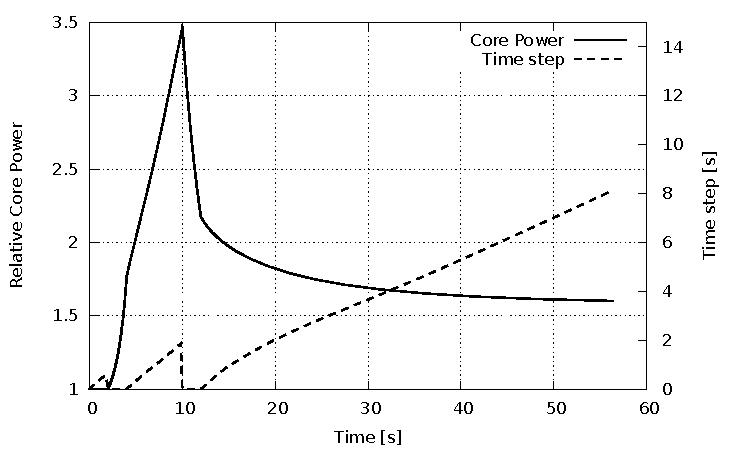
\includegraphics[scale=0.65]{figure}
\caption{\small Core Power and Time Step Response during Rod 
          Withdrawl/Insertion Transient}
\label{fig:amdahl}
\end{spacing}
\end{figurehere}
\vspace{8pt}
%

When importing figures or any graphical image please verify two things:
\begin{itemize}
\item Any number, text or symbol is in Times font and is not smaller than 
    8-point after reduction to the actual window in your paper
\item That is can be translated into PDF
\end{itemize}


Equations, such as Eq. (\ref{sample_equation}), should be centered and 
sequentially numbered to the flush right of the formula.
\begin{equation}
  \label{sample_equation}
  Speedup = \frac{1}{\frac{f}{p} + (1-f)}
\end{equation}
The continuation of a paragraph after an equation should not be indented.  
All paragraphs, as well as section or subsection headings, are separated by 
just one single empty line.


\subsubsection{Sub-section level and lower: only first character uppercase}

See Table \ref{table:example} for a sample table.  The tabls package is
recommended for improved row and column spacing.  Notice the caption appears 
above the table by setting the \texttt{$\backslash$caption} command immediately 
after the \texttt{$\backslash$begin\{table\}}. Tables are numbered in Roman 
numerals, with the caption centered above the table, in {\bf boldface}.  
Double-space before and after the table.

%
\vspace{8pt}
\begin{tablehere}
\centering
\caption{Parallel Performance for the Sample Problem}
\label{table:example}
\begin{tabular}{rccc}
 \toprule
 \multicolumn{1}{c}{Number of} & 
 Wall-Clock & 
 Speedup    & 
 Efficiency \\
 \multicolumn{1}{c}{Processors} & 
 Time$^{a}$ (min)  & 
 (T$_{s}$/T$_{p}$) & 
 (\%)              \\
 \midrule
 \midrule
 1 &  100.0 &  ---    & ---  \\
 \midrule
 2 &   52.6 &  1.9    & 95.0 \\
 \bottomrule 
\end{tabular}
\end{tablehere}
\vspace{8pt}
%

\section{Conclusions}

Present your summary and conclusions here.


\section*{Acknowledgments}

Acknowledge the help of colleagues and sources of funding, as appropriate.

The format for this template was adapted from the template for PHYSOR 2002 
posted on the Internet.  Most of the {\LaTeX} format definitions contained
in this and the accompanying files were adapted from sample files supplied 
by R. Martineau (INL), who plagiarized (adapted) the files from A. Sood 
(LANL), J. Wagner (ORNL), and James Warsa (LANL).


%\section*{References}
\setlength{\baselineskip}{12pt}

\bibliographystyle{ans}
\bibliography{references}

\end{multicols}
\end{document}
